%&xelatex
\documentclass[xcolor=svgnames]{beamer}
\usepackage[british]{babel}
\usepackage[T1]{fontenc}
\usepackage[utf8]{inputenc}
\usepackage{minted}

\usepackage{tcolorbox}
\usepackage{graphicx}
\usepackage{booktabs}

\usetheme[block=fill,progressbar=frametitle]{metropolis}
\usepackage{lmodern}

\usepackage{bytefield}

\usepackage{tikz}
\usetikzlibrary{shapes.misc, shapes.symbols, positioning, calc}

\usepackage{xcolor}
\usepackage{ulem}
\title{Control systems and Computer Networks}
\subtitle{Module Overview}

\author{Dr Alun Moon}
\date{Lecture 1.1}
\begin{document}
\frame{\maketitle}

\begin{frame}{Jacqard Loom}{Early industrial automation}
\begin{columns}[onlytextwidth]
\begin{column}{.6\textwidth}
    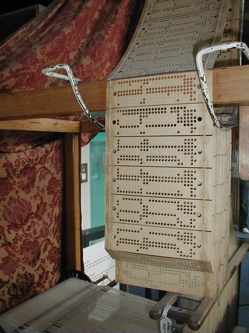
\includegraphics[height=\textheight]{Jacquard-loom-cards.jpg}
\end{column}
\begin{column}{.4\textwidth}
    \begin{itemize}
        \item Punched Cards controlling loom
        \item 1804
        \item manufacturing textiles with such complex patterns as brocade, damask and matelassé
    \end{itemize}
\end{column}
\end{columns}
\end{frame}

\newcommand\redout{\bgroup\markoverwith
{\textcolor{red}{\rule[0.3ex]{2pt}{2pt}}}\ULon}
\begin{frame}{Reality bites}
    \begin{itemize}
        \item \only<1>{Virtual}\only<2->{\redout{Virtual}} Reality
    \end{itemize}
\end{frame}

\begin{frame}{We Deal with Reality}
    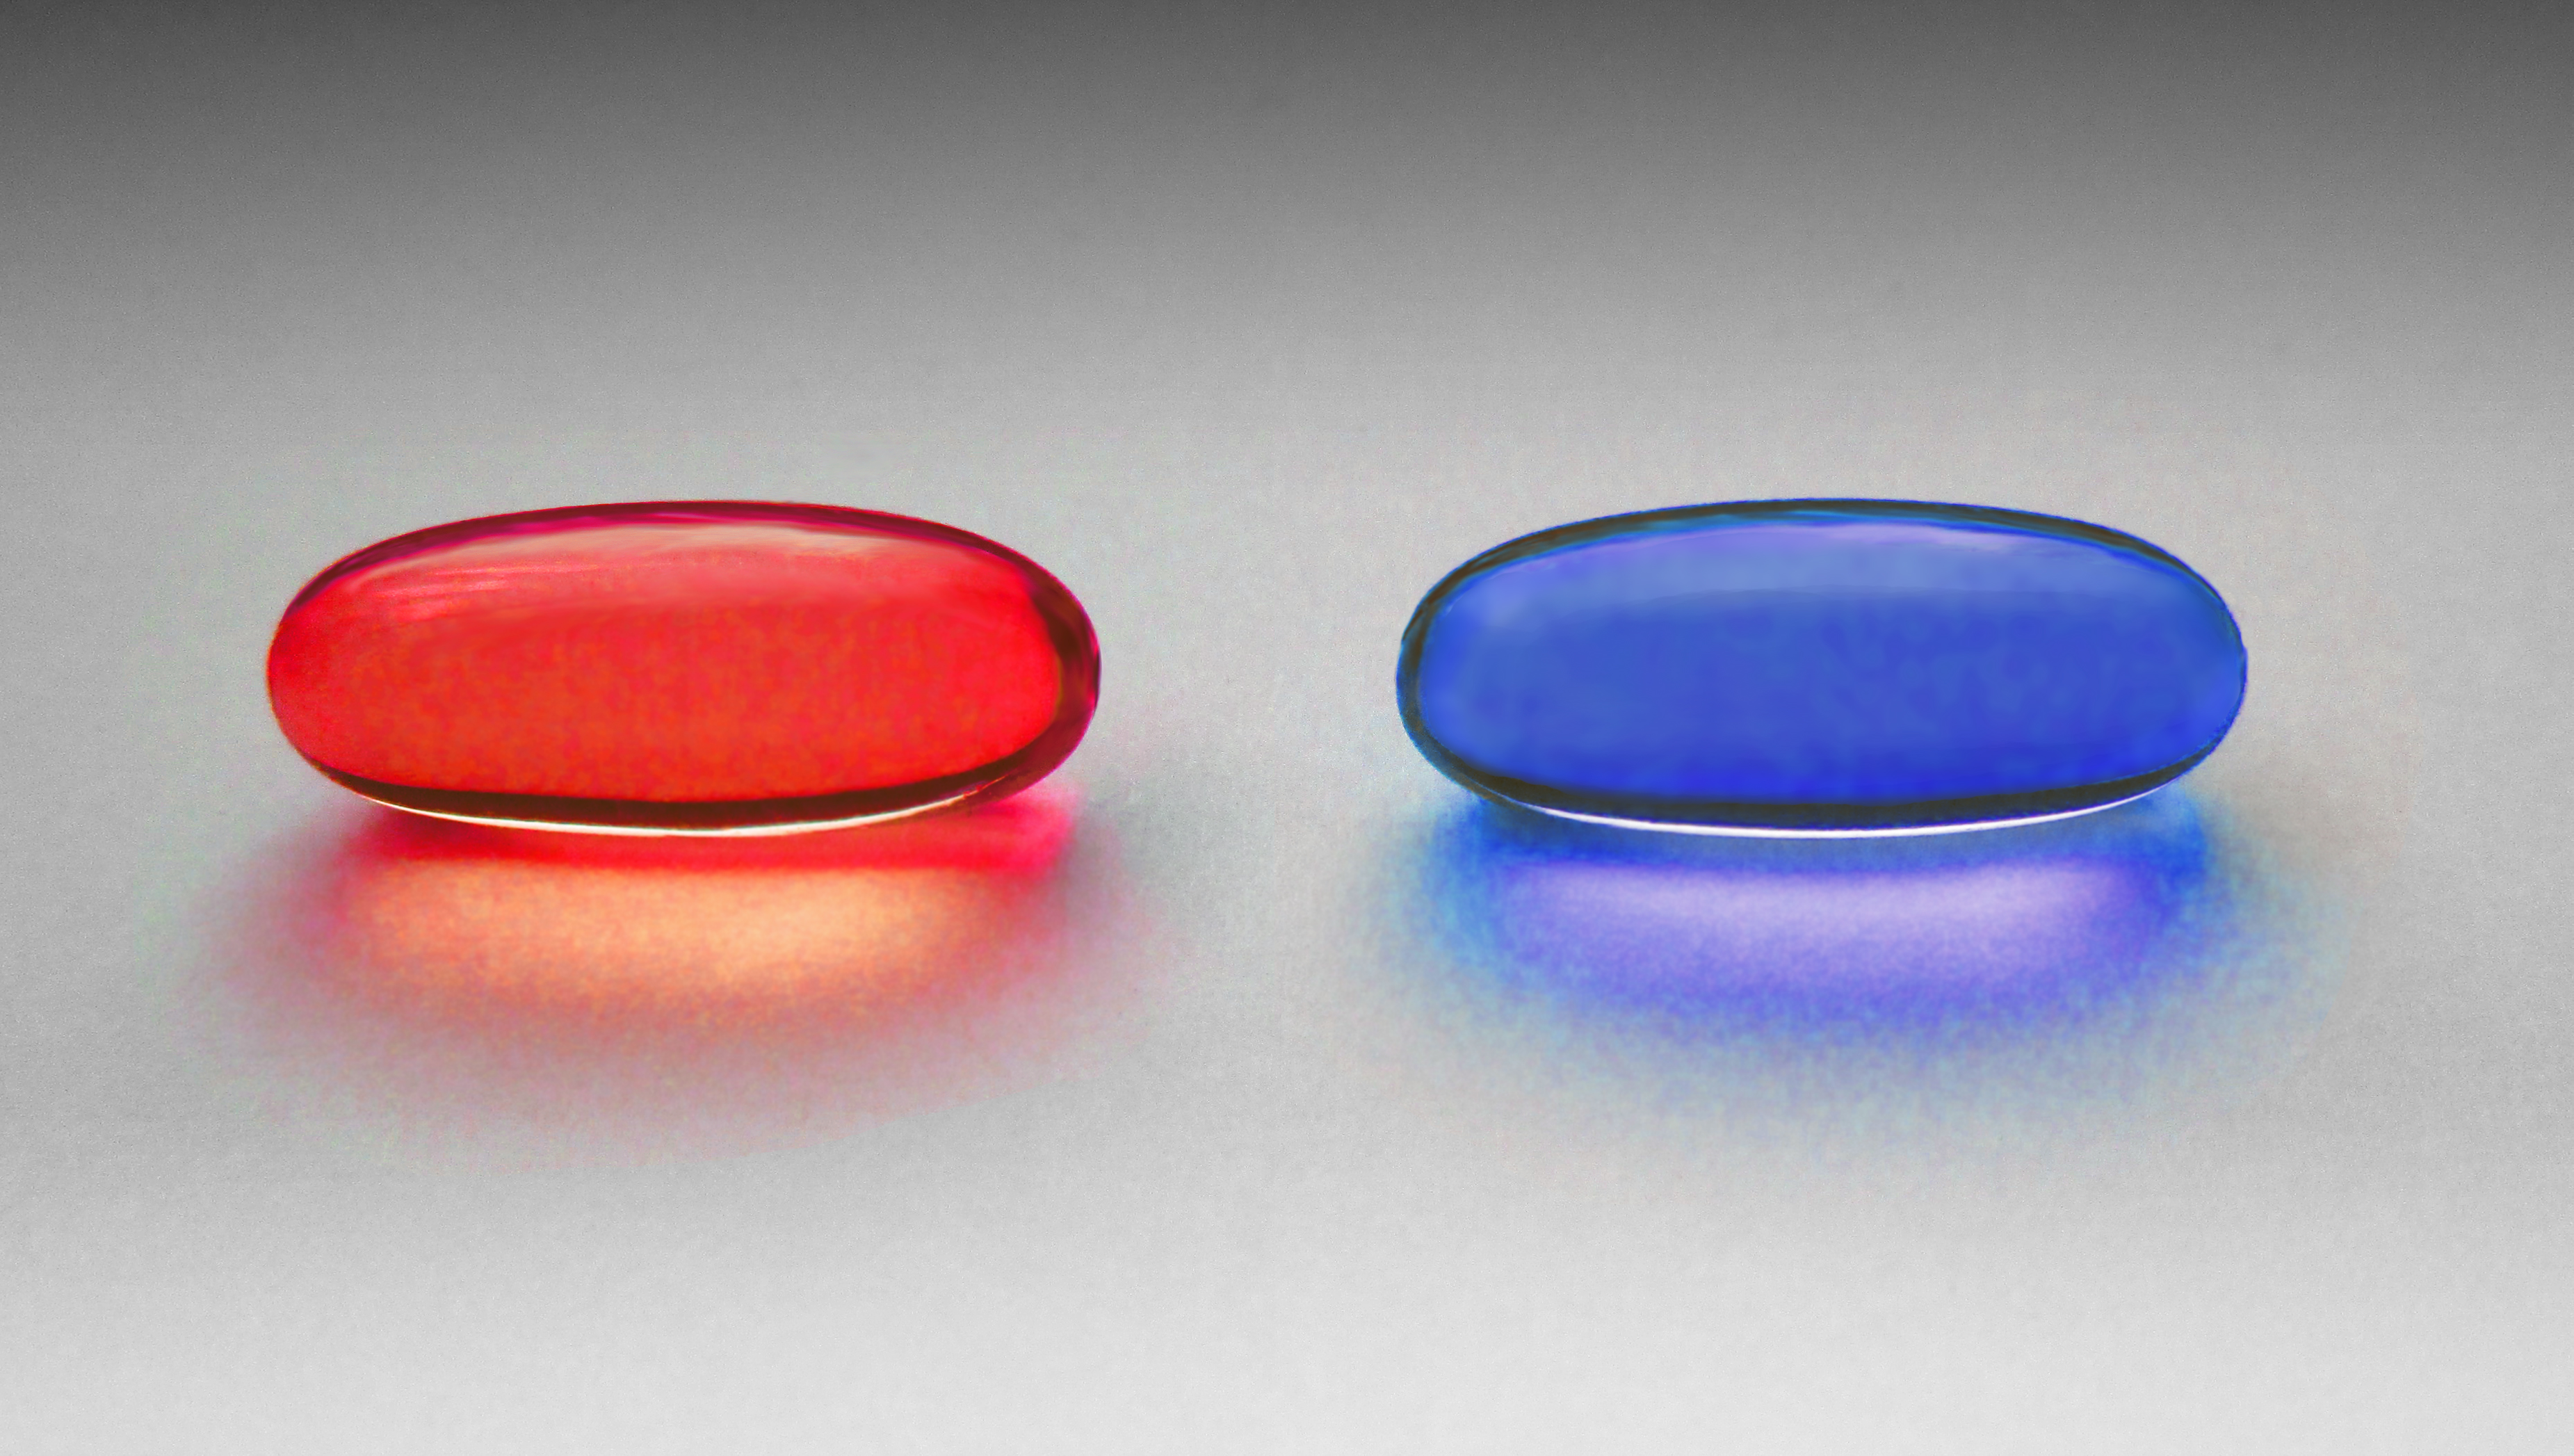
\includegraphics[width=\textwidth]{Red_and_blue_pill.jpg}
    \pause
    \begin{quote}
        You take the red pill -- you stay in Wonderland, and I show you how deep the rabbit hole goes.\\
        ~\hspace*{\fill}{\textit Morpheus, The Matrix}
    \end{quote}
    \begin{tikzpicture}[remember picture, overlay]
        \node[forbidden sign, draw, scale=8, very thick, xshift=3mm, yshift=1.2mm, line width=3mm] at (current page.center) {} ;
    \end{tikzpicture}
\end{frame}
\end{document}
%%%%======================
